%\subsection{Calcul de l'épaisseur et distance curviligne}
%Expérimentalement et numériquement, les points, représentants les profils du godet1(~\ref{fig:Step1Emboutissage}) et godet2 (~\ref{fig:Step2Emboutissage}) ont été recueillis suivant les directions de 0° à 315° avec un incrément de 45°.





%L'épaisseur locale est définie, d'après~\cite{xin_intrinsic_2016}, comme la distance entre un point
%d'un profil et son intersection avec le profil opposé, mesurée le long de la normale locale.

%La méthode se décompose en quatre étapes successives, appliquées à chaque point du profil extérieur.
%\paragraph{Étape\,1 — Calcul de la normale locale}
%\mbox{}\\
%L'épaisseur locale est mesurée perpendiculairement à la surface du godet.
%Il faut donc, pour chaque point mesuré, déterminer la direction normale au profil en ce point.
%Pour un profil discret, cette normale est estimée à partir de
%la direction reliant un point à son voisin suivant.
%On construit ainsi le vecteur tangent unitaire \(\vec{e}_1\) entre deux points
%consécutifs du profil extérieur selon la figure (~\ref{fig:normale}) :

%\noindent
%\begin{minipage}[t]{0.58\linewidth}
%\vspace{0pt}
%\[
   % \vec{e}_1 = \frac{P_{i+1}^{ext} - P_i^{ext}}{\| P_{i+1}^{ext} - P_i^{ext} \|}
  %  \tag{2}
%\]
%Le profil étant plan, la normale dans ce plan est obtenue
%par produit vectoriel avec le vecteur hors-plan \(\vec{e}_z = (0,\,0,\,1)\) :
\[
    \vec{n} = \vec{e}_1 \wedge \vec{e}_z
    \quad\Longrightarrow\quad
    \vec{n} = \begin{pmatrix} -e_{1y} \\ e_{1x} \end{pmatrix}
    \tag{3}
\]
Cette opération est répétée pour chaque point du profil, fournissant ainsi
une normale locale adaptée à la géométrie réelle (mur, rayon, fond).
\end{minipage}
\hfill
\begin{minipage}[t]{0.4\linewidth}
\vspace{0pt}
    \centering
    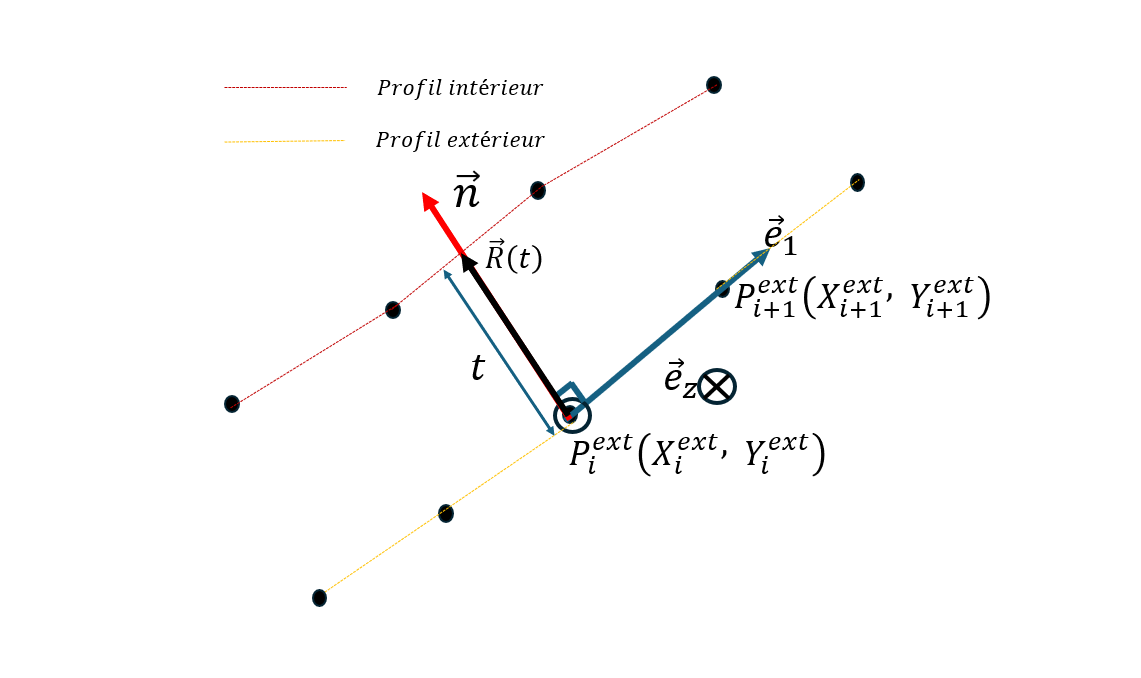
\includegraphics[width=\linewidth]{normaleeeee_Lancemeeenntt.png}
    \captionof{figure}{Normale $\vec{n}$ et lancement du rayon depuis un point du profil extérieur}
    \label{fig:normale}
\end{minipage}




%──────────────────────────────────────
\paragraph{Étape\,2 --- Lancement du rayon et recherche de l'intervalle}
\mbox{}\\
Une fois la normale connue, on lance un rayon depuis le point extérieur
\(\vec{P}_{ext} = (P_x,\,P_y)\) dans la direction \(\vec{n}\),
paramétré par la distance \(t\) selon la figure (~\ref{fig:normale}):
\begin{equation}
    \vec{R}(t) = \vec{P}_{ext} + t\cdot\vec{n}
    = \begin{cases}
        X_{ray}(t) = P_x + t\,N_x \\
        Y_{ray}(t) = P_y + t\,N_y
    \end{cases}
    \tag{4}
\end{equation}
Puisque \(\vec{n}\) est unitaire, le paramètre \(t\) est directement
l'épaisseur locale en mm. Il reste à trouver la valeur de \(t\) pour laquelle
cette projection touche le profil intérieur.

Le profil intérieur étant discret, on ne peut pas résoudre cette intersection
directement sans localiser le segment du profil intérieur
qui est traversé par cette projection normale.

\begin{wrapfigure}{r}{0.45\linewidth}
    \centering
    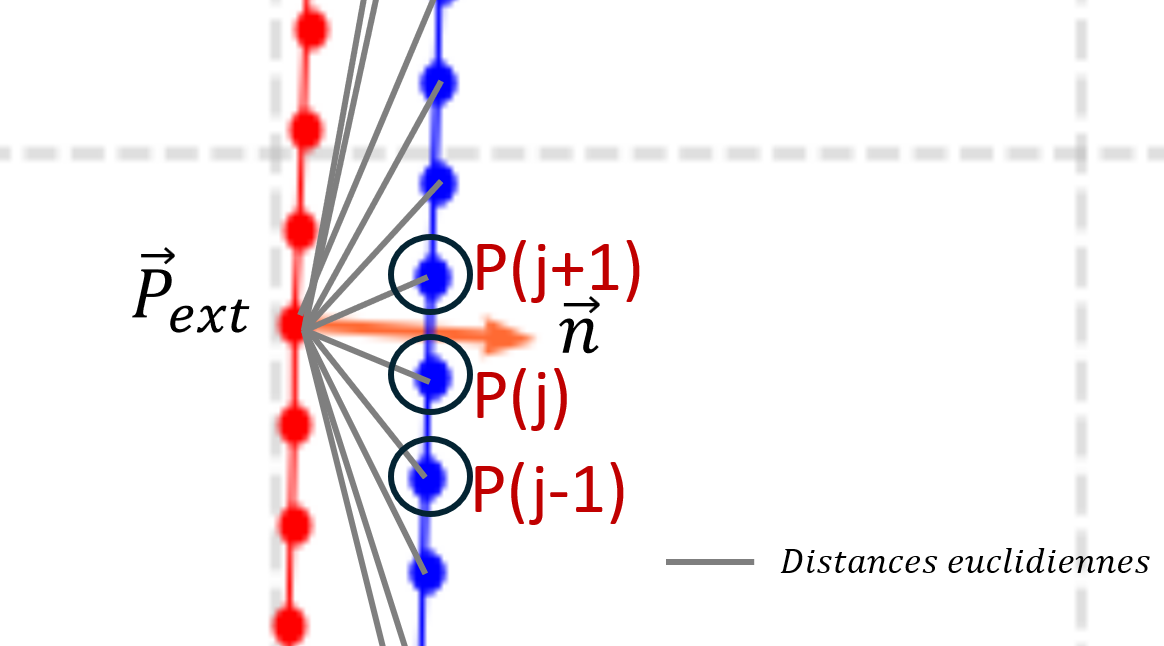
\includegraphics[width=\linewidth]{distance_euclidiennes.png}
    \caption{Distances euclidiennes entre $\vec{P}_{ext}$ et les points
    intérieurs candidats $P(j-1),\,P(j),\,P(j+1)$}
    \label{fig:distances}
\end{wrapfigure}

Pour cela, on calcule la distance euclidienne entre \(\vec{P}_{ext}\)
et chaque point intérieur \(P_j^{int}\) :
\[
    d_j^2 = \bigl(X_j^{int} - P_x\bigr)^2 + \bigl(Y_j^{int} - P_y\bigr)^2
    \tag{5}
\]
Les 3 points les plus proches \mbox{\(P(j-1)\)}, \mbox{\(P(j)\)}, \mbox{\(P(j+1)\)} sur la figure (~\ref{fig:distances}) sont retenus
comme candidats à l'intersection.
Parmi ces candidats, l'intervalle exact est identifié par le critère de colinéarité :
le rayon \(\vec{R}\) intersecte le segment \([P_j^{int},\,P_{j+1}^{int}]\)
si et seulement si \(\vec{R}\) est colinéaire à
\(\vec{u}_j = \overrightarrow{P_{ext}P_j^{int}}\),
c'est-à-dire si leur déterminant \(f_j\) s'annule.
où \((X_j,\,Y_j)\) sont les coordonnées du point intérieur \(P_j^{int}\)
et \((P_x,\,P_y)\) celles du point extérieur \(\vec{P}_{ext}\).
On calcule donc pour chaque point candidat :
\[
    f_j = \det\!\bigl(\vec{u}_j,\;\vec{n}\bigr)
        = \bigl(X_j - P_x\bigr)N_y - \bigl(Y_j - P_y\bigr)N_x
    \tag{6}
\]

Un changement de signe entre deux valeurs consécutives indique
que le rayon traverse ce segment, d'après le théorème des valeurs
intermédiaires~:
\[
    f_{j-1}\cdot f_j < 0
    \quad\Longrightarrow\quad
    \text{intersection dans }
    \bigl[P(j-1),\;P(j)\bigr]
\]

%──────────────────────────────────────
\paragraph{Étape\,3 — Résolution par égalité vectorielle}
\mbox{}\\
L'intervalle $[P(j),\,P(j+1)]$ étant identifié, le segment intérieur est
représenté de façon continue en le paramétrant par $s \in [0,1]$ :
\[
    \overrightarrow{P_j P_{j+1}}(s) = P_j + s\cdot\bigl(P_{j+1} - P_j\bigr)
    \tag{7}
\]
Le point d'intersection est la solution de l'égalité vectorielle
$\vec{R}(t) = \overrightarrow{P_j P_{j+1}}(s)$,
qui se décompose en un système linéaire $2 \times 2$ à deux inconnues
$(t,\,s)$ :
\[
    \begin{cases}
        t\,N_x - s\,(X_{j+1}-X_j) = X_j - P_x \\[4pt]
        t\,N_y - s\,(Y_{j+1}-Y_j) = Y_j - P_y
    \end{cases}
    \tag{8}
\]
La résolution fournit simultanément :
\begin{itemize}
    \item $t^* \equiv e$ : \textbf{l'épaisseur locale} (en mm),
    distance réelle entre les deux profils suivant la normale~;
    \item $s^*$ : la position du point de contact sur le segment intérieur,
    permettant de localiser précisément le point d'impact.
\end{itemize}
Ces quatre étapes sont répétées pour chacun des points du profil extérieur,
reconstituant ainsi l'évolution complète de l'épaisseur le long du godet.

%──────────────────────────────────────
\paragraph{Étape\,4 --- Représentation sur la distance curviligne médiane.}
\mbox{}\\
\begin{wrapfigure}{r}{0.4\linewidth}
    \centering
    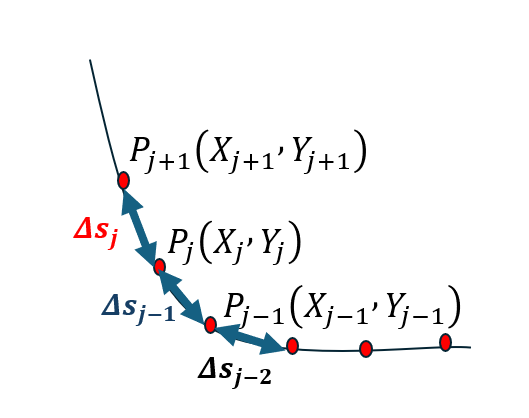
\includegraphics[width=\linewidth]{FiguresALL/Methodologie/dista_curvv.png}
    \caption{Définition de la distance curviligne}
    \label{fig:curviligne}
\end{wrapfigure}
Pour représenter l'épaisseur de façon physiquement significative et comparable
entre profils de géométries différentes, on utilise la \textbf{distance curviligne} noté \(s_j\),
qui est la longueur du chemin parcouru le long d'une courbe, calculée
point par point par la formule de Pythagore discrète (Figure~\ref{fig:curviligne}) :
{\small
\[
    \Delta s_j = \sqrt{\bigl(X_{j+1} - X_j\bigr)^2 + \bigl(Y_{j+1} - Y_j\bigr)^2}
    \tag{9}
\]
\[
    s_j = \sum_{k=0}^{j-1} \Delta s_k
    \tag{10}
\]
}
D'après les travaux de \cite{coer_mise_nodate}, cette distance curviligne
n'est pas calculée sur le profil extérieur ni sur le profil intérieur,
mais sur la \textbf{ligne médiane} --- définie comme la courbe passant
exactement à mi-épaisseur en chaque point (en rouge sur la figure~\ref{fig:mediane}) :
{\small
\[
    P_j^{med} = P_j^{ext} + \frac{t^*}{2}\,\vec{n}_j
    \tag{11}
\]
\[
    s_j^{med} = \sum_{k=0}^{j-1}
    \sqrt{\bigl(X_{k+1}^{med} - X_k^{med}\bigr)^2
    + \bigl(Y_{k+1}^{med} - Y_k^{med}\bigr)^2}
    \tag{12}
\]
}

\begin{wrapfigure}{r}{0.4\linewidth}
    \centering
    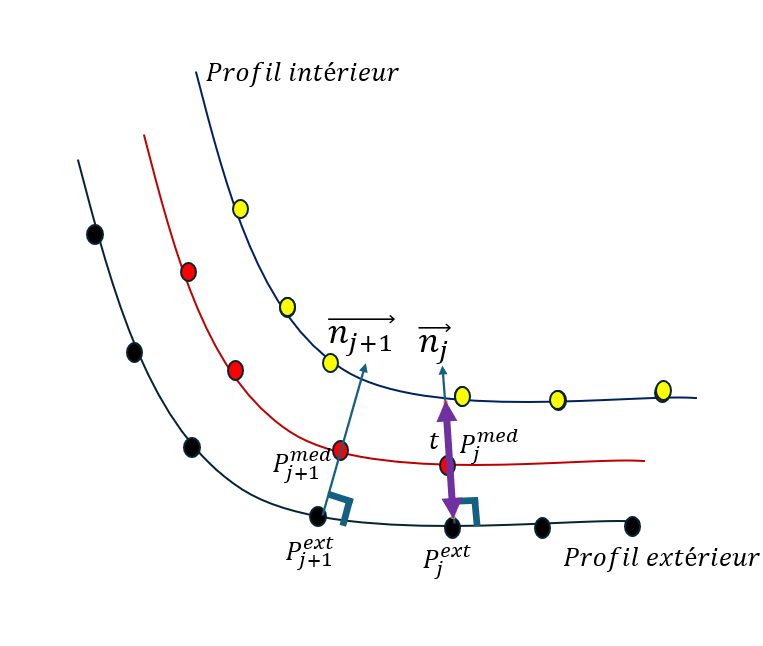
\includegraphics[width=\linewidth]{FiguresALL/Methodologie/dist_mediane.png}
    \caption{La distance curviligne médiane $s_j^{med}$}
    \label{fig:mediane}
\end{wrapfigure}

Ce choix garantit une abscisse indépendante du profil de référence
et permet une comparaison directe entre les zones du godet
(fond, rayon, mur) ainsi qu'entre différents godets.